% journal of hydrology
% !TEX TS-program = pdflatex
% !TEX encoding = UTF-8 Unicode

% This is a simple template for a LaTeX document using the "article" class.
% See "book", "report", "letter" for other types of document.

\documentclass[11pt]{article} % use larger type; default would be 10pt

\usepackage[utf8]{inputenc} % set input encoding (not needed with XeLaTeX)

%%% Examples of Article customizations
% These packages are optional, depending whether you want the features they provide.
% See the LaTeX Companion or other references for full information.

%%% PAGE DIMENSIONS
\usepackage{geometry} % to change the page dimensions
\geometry{a4paper} % or letterpaper (US) or a5paper or....
% \geometry{margin=2in} % for example, change the margins to 2 inches all round
% \geometry{landscape} % set up the page for landscape
%   read geometry.pdf for detailed page layout information

\usepackage{graphicx} % support the \includegraphics command and options

% \usepackage[parfill]{parskip} % Activate to begin paragraphs with an empty line rather than an indent

%%% PACKAGES
\usepackage{url}
\usepackage{hyperref}
\usepackage{listings}
\usepackage{booktabs} % for much better looking tables
\usepackage{array} % for better arrays (eg matrices) in maths
\usepackage{paralist} % very flexible & customisable lists (eg. enumerate/itemize, etc.)
\usepackage{verbatim} % adds environment for commenting out blocks of text & 
%for better verbatim

\usepackage{subfigure}

%\usepackage{subfig} % make it possible to include more than one captioned 
%%figure/table in a single float
% These packages are all incorporated in the memoir class to one degree or another...

%%% HEADERS & FOOTERS
\usepackage{fancyhdr} % This should be set AFTER setting up the page geometry
\pagestyle{fancy} % options: empty , plain , fancy
\renewcommand{\headrulewidth}{0pt} % customise the layout...
\lhead{}\chead{}\rhead{}
\lfoot{}\cfoot{\thepage}\rfoot{}

%%% SECTION TITLE APPEARANCE
\usepackage{sectsty}
\allsectionsfont{\sffamily\mdseries\upshape} % (See the fntguide.pdf for font help)
% (This matches ConTeXt defaults)

%%% ToC (table of contents) APPEARANCE
\usepackage[nottoc,notlof,notlot]{tocbibind} % Put the bibliography in the ToC
\usepackage[titles,subfigure]{tocloft} % Alter the style of the Table of Contents
\renewcommand{\cftsecfont}{\rmfamily\mdseries\upshape}
\renewcommand{\cftsecpagefont}{\rmfamily\mdseries\upshape} % No bold!

%%% END Article customizations

%%% The "real" document content comes below...

\title{Final Report (Draft): \\
Image Analysis using Artificial Intelligence to
Quantify the Number and Density of Mussels in Lake Erie and Ontario}

\author{Angus Galloway}
%\date{} % Activate to display a given date or no date (if empty),
         % otherwise the current date is printed
         
\pagenumbering{roman}         

\begin{document}

\maketitle

\thispagestyle{empty}

\vspace{5cm}

\begin{centering}

Report prepared for:

\vspace{1cm}

Dominique Brunet \\ 
Environment Canada \\ 
867 Lakeshore Rd \\
Burlington, ON \\
L7S 1A1 

\end{centering}

\clearpage

% an introduction, a technical discussion of the steps taken, the rationale for
% the various design choices made and parameters selected for the training of
% the computer vision model, a technical discussion summarizing the
% strengths and limitations of the computer vision model and its robustness to 
% change to change of image resolution, viewing angle and other relevant
% factors, a discussion detailing how data acquisition methods can be improved
% in future surveys, and conclusions and include, as applicable, supporting
% graphs, tables and figures.

\setcounter{page}{1}

\section*{Executive Summary}
% 250 words or less

Goes here

\clearpage

\tableofcontents

\clearpage

\pagenumbering{arabic}
\setcounter{page}{1}

\section{Introduction}

\section{Experiments} 

\subsection{Training and Testing on In-Situ Dataset}

\subsection{Training and Testing on Lab Dataset}

\subsection{Zero-Shot Generalization From In-Situ to Lab Dataset}

Figure~\ref{fig:zero-shot-situ-lab} shows model predictions that arise from
training on underwater data and evaluated on an unseen distribution of Lab
images. The generalization problem is difficult because mussels tend to sit in a
vertical orientation in the wild, with the dark gap between the two shell
halves acting as a primary visual basis for identification by human eye. 
Further, mussels tend to be darker underwater due to reduced illumination, or
from being covered with a fine layer of sediment. Conversely, Lab images are 
well illuminated and all mussels lie on their side. 

These qualitative differences between the two distributions are 
reflected in Figure~\ref{fig:zero-shot-situ-lab}. It appears that the brighter 
mussels -- which have a similar white colour as the unlabeled empty shells
underwater -- are the most prominent false positives, while the darker more 
textured area of the mussle shells are identified correctly.

\newcommand{\zshot}{./img/situ_to_lab/}

\begin{figure}
\centering
\subfigure{
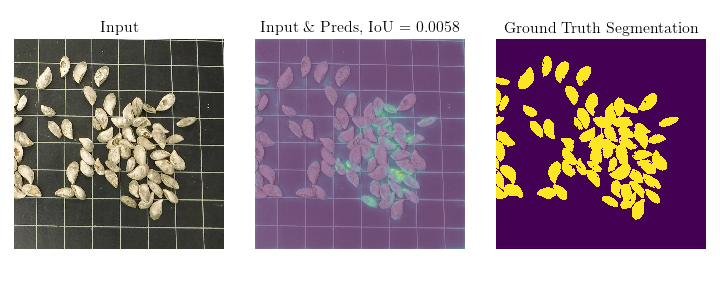
\includegraphics[width=0.9\linewidth]{\zshot/val_101-lab_100__Lab_3796-1_2018-08-13_image-1_patch_width1200__fcn8s_lr1e-03_wd5e-04_bs25_ep80_seed4_epoch70}}
\subfigure{
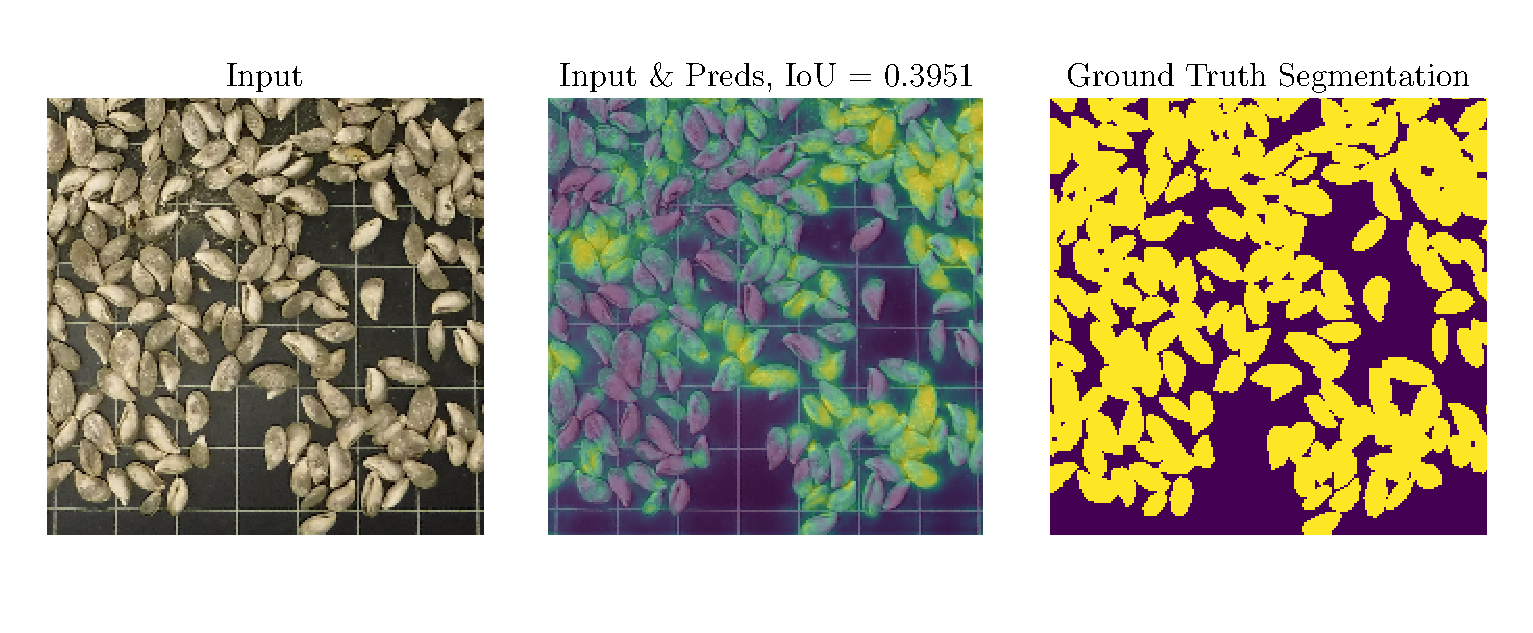
\includegraphics[width=0.9\linewidth]{\zshot/val_101-lab_100__Lab_3798-2_2018-08-13_image-1_patch_width1200__fcn8s_lr1e-03_wd5e-04_bs25_ep80_seed4_epoch70}}
\subfigure{
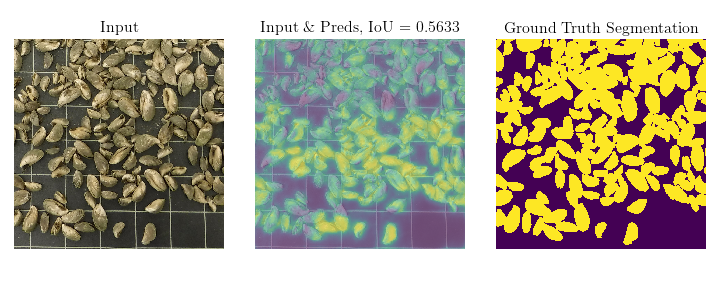
\includegraphics[width=0.9\linewidth]{\zshot/val_101-lab_100__Lab_3801-1_2018-07-11_image-1_patch_width1200__fcn8s_lr1e-03_wd5e-04_bs25_ep80_seed4_epoch70}}

\caption{Qualitative results and intersection-over-union (IoU) score arising
from training the~\texttt{FCN8s} model on~\emph{in-situ} underwater data
(\texttt{val\_v101} split) and testing on Lab data (\texttt{v100}) zero-shot. 
The first column is an input patch in RGB format, second column 
overlays the real valued sigmoid prediction score with the input, and the last 
row are the ground truth binary masks. A failure case is shown in the first
row, and more successful cases in other rows. See text for more details. 
Note: predictions are binarized for calculating IoU. All images are $1200$
square pixels for clarity.}
\label{fig:zero-shot-situ-lab}
\end{figure}

\section{Conclusion}

\section{Comparison of Data Annotation Services}

\begin{table}[]
\caption{A comparison of three image labeling services for generating ground
truth semantic segmentation masks for mussel images:
\texttt{LabelMe}~(\url{https://github.com/wkentaro/labelme}),
\texttt{Figure Eight}~(\url{https://figure-eight.com/}),
and~\texttt{Scale AI}~(\url{https://scale.com/}).
Analysis done assuming two ($C=2$) classes ``mussel'' and ``background'', but
is expected to remain consistent for $C \leq 20$. Row F) ``Latency'' means the
time elapsed between when a label is requested for a particular image and the
time it is delivered, whereas G) ``Throughput'' refers to the number of images
processed per unit time (parallelism, i.e., many workers, increases
throughput). Note: The asterisk ($^*$) for J) for~\texttt{Figure Eight} means
that the user is responsible for the creation of test examples that
automatically reject low quality judgments, otherwise the user must manually
reject them. Rejected judgments incur the same fee as accepted judgments.}
\begin{tabular}{lccc}
\toprule
Service & Manual (\texttt{LabelMe}) & \texttt{Figure Eight} & \texttt{Scale AI} 
\\ \midrule
A) Interface type & Desktop GUI & Web Interface & API Only \\ \midrule
B) Initial setup complexity \\ (Amazon MTurk = 10) & 2 & 5 & 1 \\ \midrule
C) Length of trial \\ (images labeled) & NA & 1000 (Paid) & 5 (Free) \\ \midrule
D) Minimum fee after trial & NA & 10,000 USD & NA \\ \midrule
E) Cost per image (USD) & NA & 2.25 & 6.40 \\ \midrule
F) Latency (minutes) & $1-10$ & $< 60$ & $60-240$ \\ \midrule
G) Throughput & Low & High & Medium \\ \midrule
H) Quality & High & Medium & High \\ \midrule
I) Guaranteed label for \\ all pixels & No & No & Yes \\ \midrule
J) User responsible for \\ quality assurance (QA) & Yes & Yes$^*$ & No \\  
\midrule
K) Ability to edit \\ labels in~\texttt{LabelMe} & Yes & Yes & No \\ \midrule
L) User support & Github & Email & Slack \\ 
\bottomrule
\end{tabular}
\end{table}

\subsection{Figure Eight}

Additional settings were required for good results with this platform. 
Under the Design tab, at the bottom of the page there is an option to enable 
the Code Editor. A new field ``CML'' appears in the editor, which was modified 
as follows:

\begin{lstlisting}[language=html, frame=single]
<cml:shapes label="Draw Shapes" name="annotation" 
type="['polygon']" image-url="{{image_url}}" 
polygon-threshold="0.15" class-threshold="0.1" 
ontology="true" crosshair="false" validates="required" 
class-agg="cagg_0.1" polygon-agg="0.1" gold="true"/>
\end{lstlisting}

The variables modified were: 

\begin{description}
\item[polygon-threshold] The minimum time it should take a contributor to
complete a page of work. When triggered, the contributor will be removed from
your job. Increased from default of 10 to 20 seconds.
\end{description}

These variables are documented here:\url{ 
https://success.figure-eight.com/hc/en-us/articles/360016693051-Guide-to-Polygon-Job-Design-Test-Questions-and-Aggregation}

Under Settings $>$ Contributors:

Increased the ``contributor level'' from level 1 -- \textbf{Fastest
Throughput}: All qualified contributors, to level 3 -- highest quality: 

Under Settings $>$ Quality Control:

\begin{description}
\item[Minimum Time Per Page] The minimum time it should take a contributor to
complete a page of work. When triggered, the contributor will be removed from
your job. Increased from default of 10 to 20 seconds.

\item[Results] check the box to disable responses to test questions.
\end{description}

Post processing json output from FigureEight for validation in LabelMe. We need 
to convert the report generated by FigureEight, which is in jsonstring format, 
into plain json. 

\begin{lstlisting}[language=bash, frame=single]
sed '1s/^/[/; $!s/$/,/; $s/$/]/' in.json > out.json

1  s/^/[/      # Insert a left bracket at the beginning of the first line
$! s/$/,/      # On all but the last line append a comma
$  s/$/]/      # Append a right bracket to the last line
\end{lstlisting}

\subsection{Scale AI}

This section enumerates the complete set of steps to process the output of the 
Scale AI platform for use by the python model training scripts.

\begin{enumerate}
\item Run the python
notebook~\href{https://github.com/AngusG/cciw-zebra-mussel/blob/master/labelme/scale}{postprocess-scale-labels.ipynb}
to convert the RGB colour labels from the~\texttt{Scale AI} API into the format
consistent with the~\texttt{labels.txt} file used by~\texttt{LabelMe}.

\item Run the python
notebook~\href{https://github.com/AngusG/cciw-zebra-mussel/blob/master/labelme/voc-images-and-masks-to-patch.ipynb}{voc-images-and-masks-to-patch.ipynb}
to extract small patches from each labeled image and mask for training and
validation.

\item Populate the test.txt file for VOC format:

\begin{lstlisting}[language=bash, frame=single]
user@ws1:~/Dataset/Test/GLNI/port/scale/patches$ 
ls -l *.png >> VOCdevkit/VOC2012/ImageSets/Segmentation/test.txt
\end{lstlisting}

\item Copy masks into the relevant VOCdevkit folder:

\begin{lstlisting}[language=bash, frame=single]
user@ws1:~/Dataset/Test/GLNI/port/scale/patches$ 
cp -av *.png VOCdevkit/VOC2012/SegmentationClass/
\end{lstlisting}

\item Copy jpeg images into the relevant VOCdevkit folder:

\begin{lstlisting}[language=bash, frame=single]
user@ws1:~/Dataset/Test/GLNI/port/scale/patches$ 
cp -av *.jpg VOCdevkit/VOC2012/JPEGImages/
\end{lstlisting}

\item Confirm that each folder contains the same number of images:
\begin{lstlisting}[language=bash, frame=single]
ls -l VOCdevkit/VOC2012/SegmentationClass | wc -l
ls -l VOCdevkit/VOC2012/JPEGImages/ | wc -l
\end{lstlisting}

\end{enumerate}

\subsection{Editing Segmentation Masks in GIMP}

This section outlines a procedure for editing segmentations masks that are 
already in PNG format, for example to clean up the automatically generated 
masks for the Lab images from the
notebook~\href{https://github.com/AngusG/cciw-zebra-mussel/blob/master/labelme/autolabel-lab-testing-set.ipynb}{autolabel-lab-testing-set.ipynb}.

I recommend using the~\href{https://www.gimp.org/}{GNU Image Manipulation
Program} (GIMP), which is a free and open source professional graphics program.

\begin{enumerate}
\item Select a~\texttt{*.jpg} image, right click and open with GIMP Image 
Editor.
\item In the Layers pane, select this jpg layer and click on the paint brush 
icon ``Lock pixels'' to freeze this layer.
\item From the main menu, select File, Open as Layers..., and select the PNG 
mask associated for the image.
\item Select the PNG mask from the layers pane and change the Opacity value
from $100\%$ to $50\%$.

\item To efficiently label data, I made use of the ``Free Select Tool'' from
the Toolbox, which can be enabled with the keyboard shortcut ``f''. I then fill
in the polygon drawn with the Free Select Tool using the ``Bucket Fill Tool''. 
The Bucket Fill tool default shortcut is ``Shift B'', which can be cumbersome 
when switching rapidly back and fourth. I created a new shortcut ``b'' using 
the instructions 
here:~\url{https://docs.gimp.org/2.10/en/gimp-concepts-shortcuts.html}.

\item Change the foreground color to solid red (\texttt{\#ff0000}), consistent
with the existing indexed colormap of the mussel labels, but a bit brighter to
make it easier to see which pixels have been changed in GIMP. The
notebook~\texttt{run-crf-on-gimp-masks.ipynb} ultimately merges the two red
variants into a single ``mussel'' label. Change the background color to 
black (\texttt{\#000000}). We will use this to remove any ``false positives'', 
that is, pixels predicted as mussel that should be background.

\item Under Bucket Fill, Tool Options, change ``Affected Area'' to ``Fill whole 
selection''.

\item Use the shorcut ``f'' to enable the Free Select Tool and draw the first 
polygon around a mussel. Note that you may either click to place individual
vertices, or press and hold the left mouse to draw a continous curve. Next, use
the ``b'' or ``Shift+B'' shortcut to switch to Bucket Fill. Ensure ``FG color
fill'' is selected which will use the red colour set previously for mussel. 
Similarly, to label background pixels, switch the Fill Type to ``BG color 
fill''. Repeat this step as necessary until satisfied.

\item To export a new mask in the correct format, we will now delete the JPEG 
layer. From the Layers pane, right click on the jpg file and select ``Delete
Layer''. Now select the PNG layer that we have been editing, and restore the 
Opacity to $100\%$. 

\item Select Image $\rightarrow$ Mode $\rightarrow$ Indexed from the 
main menu to change the image from RGB format to indexed color 
format. The default setting, choose optimal colormap can be 
used. For more information 
see~\url{https://docs.gimp.org/2.8/en/gimp-image-convert-indexed.html}.

\item Finally, from the File menu, Export As and append~\texttt{\_gimp.png} to 
the end of the file for reproducibility. Each Lab sample should now be 
associated with the following collection of five (5) images:

\begin{enumerate}
\item \texttt{Lab\_2907-3\_2018-07-09\_image-1.jpg} -- Original RGB JPEG image.
\item \texttt{Lab\_2907-3\_2018-07-09\_image-1\_mask\_crf.png} -- Indexed color 
PNG mask, noisy output from~\texttt{autolabel-lab-testing-set.ipynb}.
\item \texttt{Lab\_2907-3\_2018-07-09\_image-1\_mask\_crf.xcf} -- GIMP version 
of file (b) for editing.
\item \texttt{Lab\_2907-3\_2018-07-09\_image-1\_mask\_crf\_gimp.png} -- Updated 
indexed color PNG mask after processing in GIMP. Contains two shades of red, 
GIMP changes in bright red.
\item \texttt{Lab\_2907-3\_2018-07-09\_image-1\_mask\_crf\_gimp\_crf.png} -- 
After processing of file (d) with~\texttt{run-crf-on-gimp-masks.ipynb}. Contains
only a single label index, suitable for use with Python DL model training and
testing scripts.

\end{enumerate}

\end{enumerate}

\iffalse

\section{Data Acquisition}

\subsection{Field Sampling}

Divers go to specific sites (denoted by PSN code) to image and then harvest mussel samples. The diver first estimate the overall percentage coverage of mussels over the site extent. Three square quadrats (metal frames with yellow and black stripes with inside area of 0.15 squared meters) are laid down on the lake bed at three representative locations in term of mussel coverage for the site. The diver then estimates visually the percentage of live mussels (full) and the percentage of empty mussels inside each quadrat. If cladophora is present, images/videos are generally acquired before and after manual harvesting of cladophora.

Mussels are harvested by scrapping them from the lake bed surface and aspiring them in a tube. In rough water conditions, some mussels might break or be carried by the current. Divers make a visual estimate of sampling efficiency (percentage of mussels in the quadrats that are collected for analysis). Images/videos are acquired before and in some cases during the harvesting of mussels.

\subsection{Lab Analysis}
Mussels (and cladophora) are freeze-dried and brought back to the lab for analysis. The mussels are then manually counted, sorted by size with a sieve and weighted (biomass).

\subsection{Imaging Data}
Underwater video data was acquired between 2012-2018 by a hand-held camera for most of the dives. From these videos, trimmed videos were manually extracted for each portion over a quadrat. Still images were either acquired by direct image or extracted from videos. Some images were acquired by a camera system attached to a metal frame on top of quadrats (2016-2018). When multiple images were acquired for the same quadrat, the last image is deemed to be of highest quality. However, in some instances all the images available are taken before harvesting of cladophora, which might grow on top of mussels.


\section{Data Preparation}

Python scripts to generate the data described above from the data provided by WQMSD (Megan McCusker).


\subsection{Imaging Data Naming Convention}
Original video data file names were standardized to
\begin{verbatim}
f"{PSN}_{YYYY}-{MM}-{DD}.{EXT}"
\end{verbatim}
and saved on an external hard-drive in the folder
\begin{verbatim}
f"MusselsCurated/GLNI_2012-2018/GLNI_diver_videos/{PSN}/"
\end{verbatim}
In total, 493 videos were acquired for a total of 165GB of data. Format (EXT) of the videos were either .mp4, .mpg, .avi or .wmv.

Names of raw images acquired from a camera mounted on a frame were standardized to
\begin{verbatim}
f"GLNI_{PSN}-{Quadrat#}_{YYYY}-{MM}-{DD}_image-{Image#}.nef"
\end{verbatim}
and saved on an external hard-drive in the folder
\begin{verbatim}
f"MusselsCurated/GLNI_2012-2018/GLNI_quadrat_raw_images/"
\end{verbatim}
The .nef file format stands for the raw Nikon image format. In total, there are 921 raw image files taking 36.2GB of disk space.

Videos were trimmed manually by quadrat using the Windows Photo App and saved as
\begin{verbatim}
f"GLNI_{PSN}-{Quadrat#}_{YYYY}-{MM}-{DD}_video-{File#}.mp4"
\end{verbatim}
 in the folder
\begin{verbatim}
f"MusselsCurated/GLNI_2012-2018/GLNI_quadrats_stills_images_videos/"
\end{verbatim}
and subfolder
\begin{verbatim}
f"{PSN}/{YYYY}/{Mmm}.{DD}/Videos/Quad{Quadrat#}/"
\end{verbatim}
where:
\begin{description}
\item[PSN] is the diving location code.
\item[YYYY] is the four digits year.
\item[MM] is the two digits month (with leading zero).
\item[DD] is the two digits day (with leading zero).
\item[Mmm] is the first three letters of the month (with first letter capitalized).
\item[Quadrat\#] is the quadrat number (1, 2 or 3).
\item[File\#] is the video.image/still number when multiple sequences of the same quadrat were taken.
\end{description}
In addition, short videos of the metadata recorded by divers on a white board was saved in the subfolder
\begin{verbatim}
f"{PSN}/{YYYY}/{Mmm}.{DD}/Videos/Meta/"
\end{verbatim}
under the name
\begin{verbatim}
f"GLNI_{PSN}-Meta_{YYYY}-{MM}-{DD}_video-1.mp4"
\end{verbatim}
From these videos, a limited number of still images were extracted using the Windows Photo App and saved as
\begin{verbatim}
f"GLNI_{PSN}-{Quadrat#}_{YYYY}-{MM}-{DD}_still-{File#}.jpg"
\end{verbatim}
in the subfolder
\begin{verbatim}
f"{PSN}/{YYYY}/{Mmm}.{DD}/Stills/Quad{Quadrat#}/"
\end{verbatim}
Also, raw images were postprocessed with default parameters and compressed to JPEG images with quality factor 90 using a Python script. These compressed images were saved as
\begin{verbatim}
f"GLNI_{PSN}-{Quadrat#}_{YYYY}-{MM}-{DD}_image-{File#}.jpg"
\end{verbatim}
in the subfolder
\begin{verbatim}
f"{PSN}/{YYYY}/{Mmm}.{DD}/Images/Quad{Quadrat#}/"
\end{verbatim}
For this project, the difference between "stills" and "images" is the source: stills are extracted from video files while images are taken directly from a camera. In total, there are 2089 trimmed video, compressed images or video still files taking a total of 14.6GB of space.


\subsection{Table Data}

The source Excel spreadsheet obtained from Megan McCusker of the Water Quality Monitoring and Surveillance Division (WQMDS) is stored in the external hard-drive as
\begin{verbatim}
"GLNI_Miussel_Analysis_Data_2012-2018.xlsx"
\end{verbatim}
in the folder
\begin{verbatim}
f"MusselsCurated/Tables/"
\end{verbatim}

This spreadsheet was reformatted into three tables: "Sites.csv", "Dives.csv" and "Analysis.csv". The "Sites.csv" table contains the following columns:
\begin{description}
\item[PSN] Unique code for site identification
\item[Lake] Name of lake
\item[Name] Name of site
\item[Latitude] decimal latidunal (North-South) position (GPS coordinates)
\item[Longitude] decimal longitidunal (East-West) position (GPS coordinates)
\end{description}
The Sites table is extracted from the "site names" sheet in the source Excel spreadsheet. The following entries were added under "ERIE SITES" to represent locations for "Nanticoke Shoal" (July 19, 2016 dive):
\[
\begin{array}{llll}
PSN & Latitude & Longitude & Name \\
502	& 42.7728 &	-79.9694	& Peacock Point\\
504	& 42.7881 &	-79.9838	& Peacock Point
\end{array}
\]
Note: the "Name" field in the "Sites.csv" table should be changed to "Site Name" to avoid confusion with "Name" field from images, videos or stills.

The "Dives.csv" table contains information that stays constant for a given dive at a specific site and day. It includes the following columns:
\begin{description}
\item[Dive Index] Unique index for the dive
\item[CSN] Code for dive number (unique for each dive index)
\item[Cruise \#] Code for the cruise (not-unique)
\item[PSN] Code for site identification (match PSN from "Sites.csv")
\item[Date] Date of the dive (YYYY-MM-DD)
\item[Depth (m)] Depth of water at the site
\item[Overall Coverage] Percentage mussel coverage at the site as visually estimated by diver
\item[Silt (\%)]	1/512 mm to 1/64 mm in diameter.
\item[Clay (\%)	] Less than 1/512 mm in diameter.
\item[Sand (\%)] 1/16 to 2 mm in diameter.
\item[Gravel (\%)] 2 to 64 mm in diameter.
\item[Cobble (\%)] 64 to 256 mm in diameter.
\item[Rock (\%)] Not clear, maybe something of size between cobble and boulders.
\item[Bedrock (\%)] Underlying hard rock structure.
\item[Boulders (\%)] Greater than 256 mm in diameter.
\item[Shale (\%)] Underlying brittle rock structure.
\item[Underlying Substrate Type] Type of rock found under the sediments.
\item[Underlying Substrate Depth (cm)] Depth under lake bed.
\end{description}
Note that each substrate type was independently visually estimated by the diver, so the total percentage does not always add up to 100\%.

The "Analysis.csv" table contains information pertaining to a particular quadrat, which is a square metal frame of area of $0.15 m^2$. It contains the following columns:
\begin{description}
\item[Analysis Index] Unique index for the analysis.
\item[Dive Index] Index of the dive associated with the analysis.
\item[Quadrat] Quadrat number (unique for each dive index).
\item[LiveCoverage] Percentage of area with live (full) mussels within the quadrat as visually estimated by diver.
\item[EmptyCoverage] Percentage of area with empty/broken mussels within the quadrat.
\item[Biomass] Total mass (g) of mussels tissue within the quadrat as measured in the lab.
\item[Count] Total number of live mussels within the quadrat as counted in the lab.
\item[Xmm] Percentage of mussels not passing the X mm sieve (estimated mussel size of more than X mm in diameter).
\end{description}
Sieve sizes are 16 mm, 14 mm, 12.5 mm, 10 mm, 8 mm, 6.3 mm, 4 mm and 2 mm. Note that in some cases, the sum of live and empty coverage exceeds 100\%. This inconsistency might either due to errors in estimation of the coverage or by considering live mussels underneath empty shells.

The "FullVideos.csv" table links video names with "Dive Index". The "Video Name" column, which corresponds to the basename of each video file, serves as a unique index. It is associated with the "Dive Index" using the PSN number and the date. Finally, "Video Path" corresponds to the full file path of the original (names not curated) video file. It should eventually be changed to the file path of the standardized video files. Eventually, more metadata could be added in the table, such as file size, video duration, frame rate and frame resolution.

The "QuadratVideos.csv" (and "QuadratStills.csv") tables links trimmed video files (extracted stills) per quadrat to an "Analysis Index". It contains the folllowing columns:
\begin{description}
\item[Source Video] The basename of the full video from which the trimmed video (stilll) was extracted. It corresponds to "Video Name" in the "Fullvideos.csv" table.
\item[Name] The basename of the trimmed (per quadrat) video file.
\item[Quadrat Video Path] The full path to the trimmed video (in the external hard-drive, not in the Google Drive). For "QuadratVideos.csv" only.
\item[Quadrat Still Path] The full path to the still (in the external hard-drive, not in the Google Drive). For "QuadratStills.csv" only.
\item[Analysis Index] The index of the anlaysis associated with the trimmed video. It is found from the PSN, date and quadrat number.
\end{description}

The "ImageTable.csv" table links raw images to the "Analysis Index". It contains the folllowing columns:
\begin{description}
\item[Analysis Index]
\item[Raw Image Path] The raw image path in the external hard-drive.
\item[Name] The basename of the raw image path.
\item[Timestamp] The timestamp when the image was acquired, as recorded in image metadata.
\end{description}
Note that compressed images (.jpg) are stored in the Google Drive. The "ImageTable.csv" is assembled in three steps. First, a table is made from image names from 2017-2018. A second table for images from 2016 (without quadrat information) is populated, with quadrat information manually inputed. Finally, the two tables are merged into "ImageTable.csv".

The Google Colab Notebook "ImagingDataInventory.ipynb" compares the imaging data listed in "ImageTable.csv", "QuadratVideos.csv" and "QuadratStills.csv" with the imaging data stored in the Google Drive. The list of file names for which any difference is found is returned for each of the three tables. As all imaging data is updated on the Google Drive, the difference should be an empty set.


\subsection{Merging Tables}

The Google Colab Notebook "TableDataPreparation.ipynb" generates two merged tables: a large un-processed "MergedTable.csv" and a smaller pre-processed "SimplifiedImagingAnalysis.csv".

The "MergedTable.csv" table is assembled in two steps. A first table is obtained by merging "Analysis.csv" and "Dives.csv" on "Dive Index" and then merging the resulting table with "Sites.csv" on "PSN". This first table contains all the data analysis information. A second table is generated by appending "ImageTable.csv", "QuadratVideos.csv" and "QuadratStlls.csv" (which share the "Name" field). This second table links all imaging information to the "Analysis Index". The two tables are then merged on "Analysis Index"  to generate "MergedTable.csv". Note that "Name" has to be changed to "Site Name" in "Sites.csv" to differentiate from the "Name" column in the other tables. The merged table should be used in a read-only mode as it has multiple redundant information spread out through many rows.

For the "SimplifiedImagingAnalysis.csv" table, a single imaging data per analysis is selected. Pre-processing steps include:
\begin{itemize}
\item Replacing null values to 0 for "Shale (\%)" in "Dives.csv"
\item Replacing null values of "Live Coverage" in "Analysis.csv" to the corresponding "Overall Coverage" value from "Dives.csv"
\item Replacing percentage values to count for mussel size by replacing null values to "0" in "Xmm" column and by multiplying "Xmm" column with "Count" column in "Analysis.csv".
\end{itemize}
The last imaging data available is selected for each "Analysis Index" with order of preference: i) raw images, ii) quadrat videos, iii) stills. Only a subset of columns useful for image analysis are kept.


\section{Table Data Exploration}

The Google Colab Notebook "TableDataExploration.ipynb" generates statistics and summaries for different columns of table data.  In particular, it displays the diving sites on a map, count the number of dives and boat cruises per day, per month and per year, and displays histograms for mussels count, biomass, size distribution, depth, and substrate type percentage. Finallly, it provides a count for the number of analysis and the number of analysis with associated imaging data and the number of unique analysis associated with imaging data.


The Google Colab Notebook "TableDataAnalysis.ipynb" performs a correlation analysis between different columns of table data.

\fi

\end{document}
